\documentclass[12pt]{article}

\title{\vspace{-3em}PHYS 161a HW 03}
\author{Michael Cardiff}
\date{\today}

%% science symbols 
\usepackage{amsmath}
\usepackage{amssymb}
\usepackage{physics}
\usepackage{slashed}

%% general pretty stuff
\usepackage{bm}
\usepackage{enumitem}
\usepackage{float}
\usepackage{graphicx}
\usepackage[margin=1in]{geometry}
\usepackage[labelfont=bf]{caption}
\usepackage{tikz}

% figures
\graphicspath{ {./figs/} }

\renewcommand{\L}{\mathcal{L}}
\newcommand{\D}{\partial}
\newcommand{\F}{\mathcal{F}}
\newcommand{\mcD}{\mathcal{D}}

\newcommand{\vphi}{\varphi}
\newcommand{\vtphi}{\tilde{\varphi}}
\newcommand{\eps}{\epsilon}
\newcommand{\munu}{{\mu\nu}}
\newcommand{\sla}[1]{\slashed{#1}}
\newcommand*\circled[1]{\tikz[baseline=(char.base)]{
    \node[shape=circle,draw,inner sep=2pt] (char) {#1};}}

\begin{document}
\maketitle
\section{Concentric Shells}
This variation on Coulomb's law would lead to the following potential for a single point charge on the origin:
\begin{align*}
  \vphi(r)=\frac{Q}{4\pi\varepsilon_0}\frac1{1+\epsilon}\frac1{r^{1+\eps}}
\end{align*}
Similarly to how we derived in class, the formula for the potential at any point $p$ is:
\begin{align*}
  \vphi(p)=\int\dd{V'}\frac{\rho(\vb{r}')}{\abs{\vb{r-r}'}^{1+\eps}}
\end{align*}
For a shell, we have a surface charge density spread across the surface of the sphere, such that
\begin{align*}
  \rho_{shell}=\frac{\sigma}{4\pi a^2}\delta(r-a)
\end{align*}
The relevant coordinates which will be used from here on out are defined here:
\begin{figure}[H]
  \centering
  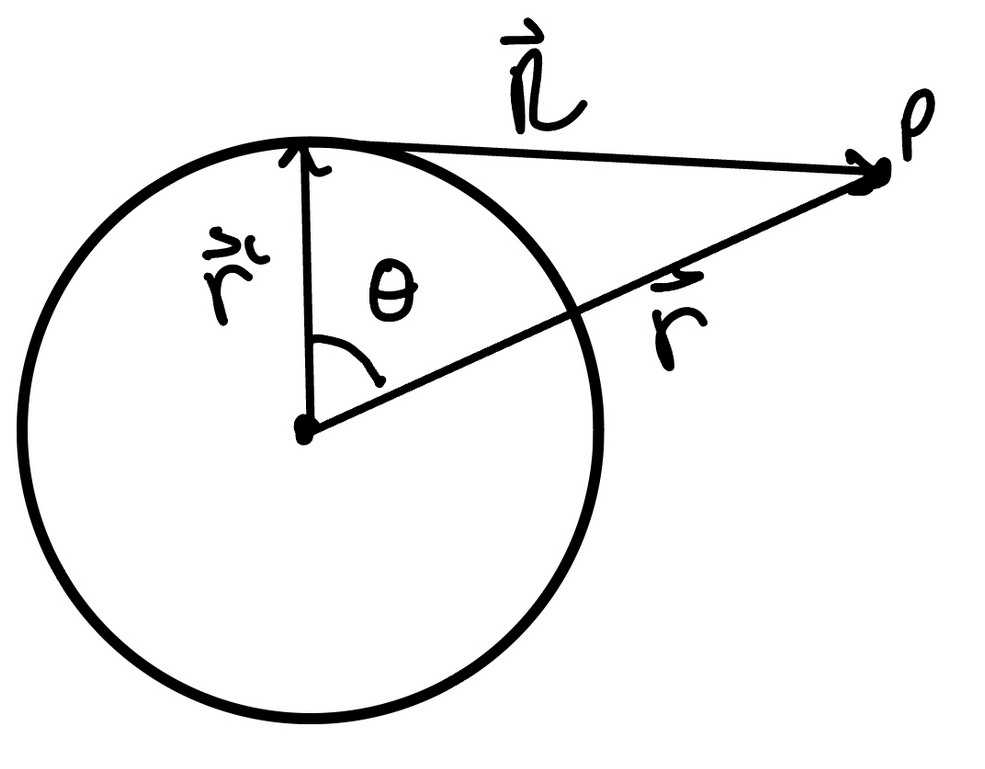
\includegraphics[width=8.0cm]{coords}
  \caption{Coordinates that are used from here on}
\end{figure}
Where the circle is of radius $a$. The integral using these conventions is
\begin{align*}
  \vphi&=\frac{\sigma}{16\pi^2 \varepsilon_0a^2}
  \int_0^{2\pi}\dd{\phi}\int_0^{\pi}\dd{\theta}\frac{a^2}{1+\eps}
  \frac{\sin\theta}{R^{1+\eps}}\\
  &=\frac\sigma{16\pi^2\varepsilon_0(1+\eps)}
  \int_0^{2\pi}\dd{\phi}\int_0^{\pi}\dd{\theta}\frac{\sin\theta}{R^{1+\eps}}
\end{align*}
We know from before that we can write the following:
\begin{align*}
  R^2=a^2+r^2-2ar\cos\theta
\end{align*}
Taking a differential:
\begin{align*}
  R\dd{R}=ar\dd{(\cos\theta)}
\end{align*}
If we notice above $\sin\theta\dd{\theta}=\dd{(\cos\theta)}$, we can also integrate out $\phi$ to get:
\begin{align*}
  \frac\sigma{8\pi ar\varepsilon_0(1+\eps)}
  \int_{r_1}^{r_2}\frac{\dd{R}}{R^\eps}
\end{align*}
Define the constant in front of the integral to be $\gamma$:
\begin{align*}
  \beta=\frac\sigma{8\pi ar\varepsilon_0(1+\eps)}
\end{align*}
The integral can be evaluated as
\begin{align*}
  \beta\int_{r_1}^{r_2}R^{-\eps}\dd{R}=\frac\beta{1-\eps}
  \qty(r_2^{1-\eps}-r_1^{1-\eps})
\end{align*}
We want to solve in terms of a charge, so we should now write the constant $\beta$ in terms of the charge and a new constant $\alpha$:
\begin{align*}
  \frac\beta{1-\eps}=\frac\sigma{4\pi a^2}\qty(\frac{a}{2r\varepsilon_0(1+\eps^2)})=\frac{Q}{r}\alpha(a)
\end{align*}
Thus the potential of a shell is:
\begin{align*}
  \vphi_{shell}(r)=\alpha(a)\frac{Q}r\qty(r_2^{1-\eps}-r_1^{1-\eps})
\end{align*}
We can the $r_i^{1-\eps}$ in powers of $\eps$:
\begin{align*}
  r_i^{1-\eps}=r_i-r_i\ln(r_i)
\end{align*}
Thus the field for a shell is:
\begin{align*}
  \vphi_{shell}(r)=\alpha(a)\frac{Q}r\qty(r_2-r_1+r_1\ln(r_1)-r_2\ln(r_2))
\end{align*}
Since $r_1,r_2$ are defined by $\theta=0,\pi$ respectively, we have the following conditions:
\begin{align*}
  r_1&=
  \begin{cases}
    r-a & \text{Outside shell}\\
    0 & \text{On Shell}\\
    a-r & \text{Inside shell}
  \end{cases}\\
  r_2&=r+a
\end{align*}
The potential for $2$ shells is then going to be:
\begin{align*}
  \vphi_{shell\,a}&=\vphi_{aa}+\vphi_{ab}\\
  \vphi_{shell\,b}&=\vphi_{bb}+\vphi_{ba}
\end{align*}
However for all intents and purposes, we are interested in the difference of the potentials, so $\phi_{ab}=\phi_{ba}$ so we can take it to be $0$:
\begin{align*}
  \vphi_a(a)+\vphi_b(a)=\alpha(b)\frac{Q_b}a\qty((a+b)(1-\ln(a+b))
  -(b-a)(1-\ln(b-a)))\\
  \vphi_a(b)+\vphi_b(b)=\alpha(a)\frac{Q_a}b\qty((a+b)(1-\ln(a+b))
  -(b-a)(1-\ln(b-a)))
\end{align*}
These should be equal in equilibrium:
\begin{align*}
  \vphi_a(a)+\vphi_b(a)=\vphi_a(b)+\vphi_b(b)
\end{align*}
I am not sure where to go from here, However clearly the multiplication cancels out, so we get proportionality of:
\begin{gather*}
  \alpha(b)bQ_b=\alpha(a)aQ_a\\
  \frac{b^2}{2\varepsilon_0(1+\eps^2)}Q_b=
  \frac{a^2}{2\varepsilon_0(1+\eps^2)}Q_a
\end{gather*}
Clearly I messed up somewhere, but I am too tired to try to figure out where, so I give up
\section{Parallel Field Components}
The electric field is defined in terms of the inside and outside of the surface:
\begin{align*}
  \vb{E}=\vb{E}_1(\vb{r})H(f)+\vb{E}_2(\vb{r})H(-f)
\end{align*}
Where the surface is defined as $f=0$ as told in the problem.

The relevant Maxwell equation to use is the curl of $\vb{E}$ since we need the components of $\vb{E}$ projected onto a tangent plane, so we need to get a cross product with the unit normal vector $\vu{n}$, taking a curl on both side:
\begin{align*}
  \curl{\vb{E}}=\curl{(\vb{E}_1(\vb{r})H(f))}+\curl{(\vb{E}_2(\vb{r})H(-f))}
\end{align*}
Using the curl of a scalar times a vector identity:
\begin{align*}
  \curl{(\psi\vb{A})}=\psi\qty(\curl{\vb{A}})+(\grad{\psi})\times\vb{A}
\end{align*}
We already have that $\curl{\vb{E}}=0$ due to the Maxwell Equation, the rest is:
\begin{align*}
  0=(\curl{\vb{E}_1})H(f)+(\grad{H(f)})\times\vb{E}_1
  +(\curl{\vb{E}_2})H(-f)+(\grad{H(-f)})\times\vb{E}_2
\end{align*}
We can eliminate the other two curls using the Maxwell Equation again, and we are left with:
\begin{align*}
  0=(\grad{H(f)})\times\vb{E}_1
  +(\grad{H(-f)})\times\vb{E}_2
\end{align*}
The gradient vector is going to be in the direction of steepest ascent, which is the normal vector of the surface $f$, and the derivative of a heaviside function is a delta:
\begin{align*}
  0&=(\vu{n}\delta(f))\times\vb{E}_1-(\vu{n}\delta(f))\times\vb{E}_2\\
  &=\delta(f)\vu{n}\times\vb{E}_1-\delta(f)\vu{n}\times\vb{E}_2
\end{align*}
The $\delta$ can be ignored as they are the same, leaving us with the following:
\begin{align*}
  0&=\vu{n}\times\vb{E}_1-\vu{n}\times\vb{E}_2\\
  &=\vu{n}\times\qty(\vb{E}_1-\vb{E}_2)
\end{align*}
This represents any vector that is perpendicular to the normal vector, which is in the tangent plane of the surface, also known as the parallel components:
\begin{align}
  \boxed{\vb{E}_1^{\parallel}-\vb{E}_2^{\parallel}=0}
\end{align}
Which means that the parallel components are continuous
\section{Damped Harmonic Oscillator}
We want to solve for $G(t)$ from the following differential equation:
\begin{align*}
  \qty(\dv[2]{t}+2\lambda\dv{t}+\omega_0^2)G(t)=\delta(t)
\end{align*}
Notate the Fourier Transform by $\F$, we wish to solve for $G(t)$ by taking the inverse transform of:
\begin{align*}
  \ip{\F\qty[\qty(\dv[2]{t}+2\lambda\dv{t}+\omega_0^2)G(t)]}{\vtphi(\omega)}=
  \ip{\F\qty[\delta]}{\vtphi(\omega)}
\end{align*}
Define the differential operator in the parentheses as $\mathcal{D}$:
\begin{align*}
  \ip{\F[\mcD(t)G(t)]}{\vtphi(\omega)}=\ip{\F[\delta]}{\vtphi(\omega)}
\end{align*}
Denote the fourier transform of $\vtphi(\omega)$ as $\vphi(t)$:
\begin{align*}
  \ip{\F[\mcD(t)G(t)]}{\vtphi(\omega)}=
  \ip{\mcD(t)G(t)}{\F[\vtphi(\omega)]}=
  \ip{\mcD(t)G(t)}{\vphi(t)}
\end{align*}
The function $\vphi(t)$ is defined as:
\begin{align*}
  \vphi(t)=\int_{-\infty}^\infty\dd{\omega}\vtphi(\omega)
  e^{i\omega t}
\end{align*}
Take the first term of the differential operator $\mcD(t)$:
\begin{align*}
  \ip{\dv[2]{G(t)}{t}}{\vphi(t)}\equiv\ip{G(t)}{\vphi''(t)}
\end{align*}
This is:
\begin{align*}
  \dv[2]{\vphi(t)}{t}=\dv[2]{t}\qty(
  \int_{-\infty}^\infty\dd{\omega}\vtphi(\omega)e^{i\omega t})
\end{align*}
We can pull the total derivative into the integral as a partial:
\begin{align*}
  \dv[2]{t}\qty(
  \int_{-\infty}^\infty\dd{\omega}\vtphi(\omega)e^{i\omega t})&=
  \int_{-\infty}^\infty\dd{\omega}\vtphi(\omega)
  \pdv[2]{t}e^{i\omega t}\\ &=
  \int_{-\infty}^\infty\dd{\omega}\qty(-\omega^2\vtphi(\omega))
  e^{i\omega t}\\
  &=\F[-\omega^2\vtphi]
\end{align*}
We can then identify:
\begin{align*}
  \ip{G(t)}{\vphi''(t)}=\ip{G(t)}{\F[-\omega^2\vtphi]}=
  \ip{\F[G(t)]}{-\omega^2\vtphi}=\ip{-\omega^2\F[G(t)]}{\vtphi}
\end{align*}
The next term is:
\begin{align*}
  \ip{2\lambda\dv{G(t)}{t}}{\vphi(t)}=-2\lambda\ip{G(t)}{\vphi'(t)}
\end{align*}
Doing the same work as before:
\begin{align*}
  \dv{\vphi(t)}{t}&=\dv{t}\qty(
  \int_{-\infty}^\infty\dd{\omega}\vtphi(\omega)e^{i\omega t})\\
  &=\int_{-\infty}^\infty\dd{\omega}
  \vtphi(\omega)\pdv{t}\qty(e^{i\omega t})\\
  &=\int_{-\infty}^\infty\dd{\omega}
  \qty(i\omega\vtphi(\omega)) e^{i\omega t}=\F[i\omega\vtphi]
\end{align*}
Once again:
\begin{align*}
  -2\lambda\ip{G(t)}{\vphi'(t)}&=-2\lambda\ip{\F[G(t)]}{i\omega\vtphi}\\
  =-2\lambda\ip{i\omega\F[G(t)]}{\vtphi}&=\ip{-2i\lambda\omega\F[G(t)]}{\vtphi}
\end{align*}
And the final term is simple since the constant just carries through like the intermediate steps before:
\begin{align*}
  \ip{\omega^2G(t)}{\vphi(t)}=\ip{\omega_0^2\F[G(t)]}{\vtphi}
\end{align*}
Hence we have:
\begin{align*}
  \ip{\mcD(t)G(t)}{\vphi(t)}=
  \ip{\qty(\omega_0^2-\omega^2-2i\lambda\omega)\F[G(t)]}{\vtphi(\omega)}
\end{align*}
The Fourier transform of the delta is just the unit operator, so we can identify the following algebraic equation:
\begin{align*}
  (\omega_0^2-\omega^2-2i\lambda\omega)\F[G(t)]=1
\end{align*}
Hence the Fourier Transform of $G(t)$ is:
\begin{align*}
  \F[G(t)]=\frac1{\omega_0^2-\omega^2-2i\lambda\omega}
\end{align*}
Applying the inverse transform as given in class:
\begin{align*}
  G(t)&=\frac1{2\pi}\int_{-\infty}^\infty
  \dd{\omega}\tilde{G}(\omega)e^{-i\omega t}\\
  &=\frac1{2\pi}\int_{-\infty}^\infty\dd{\omega}
  \frac{e^{-i\omega t}}{\omega_0^2-\omega^2-2i\lambda\omega}
\end{align*}
However we are given the condition that $G(t)=0$ for $t<0$. We can solve this integral using complex analysis and the residue theorem, note that the following singularities are in the denominator:
\begin{align*}
  \omega=-i\lambda\pm\sqrt{-\lambda^2+\omega_0^2}
\end{align*}
The residue at either point is:
\begin{align*}
  \mathrm{Res}=\pm\frac{e^{t\qty(-\lambda \pm i\sqrt{\omega_0^2-\lambda^2})}}
  {2\sqrt{\omega_0^2-\lambda^2}}
\end{align*}
The positive residue will be the one which satisfies the boundary condition, so we choose the contour which selects that one, giving:
\begin{align}
  \boxed{G(t)=\frac{e^{t\qty(-\lambda+i\sqrt{\omega_0^2-\lambda^2})}}
  {2\sqrt{\omega_0^2-\lambda^2}}}
\end{align}
\section{Potential}
We can find the potential from the charge density using the following integral
\begin{align*}
  \vphi(\vb{r})=\frac1{4\pi\varepsilon_0}\int\dd[3]{r'}
  \frac{\rho(\vb{r}')}{\abs{\vb{r-r}'}}
\end{align*}
With the charge density:
\begin{align*}
  \rho(\vb{r})=\alpha(R-r)\qty(1-\cos\theta)^2
\end{align*}
and is $0$ for $\abs{\vb{r}}>R$.

We can rewrite the $\vb{r-r}'$ with $\vb{r}'$ oriented along the $z$ axis:
\begin{align*}
  \abs{\vb{r-r}'}=\sqrt{r^2+(r')^2-2rr'\cos\theta'}
\end{align*}
Thus the integral is given as:
\begin{align*}
  \vphi(\vb{r})=\frac\alpha{4\pi\varepsilon_0}
  \int_0^{2\pi}\dd{\phi'}
  \int_0^\pi\dd{\theta'}\sin\theta'
  \int\dd{r'}(r')^2\frac{(R-r')\qty(1-\cos\theta')^2}
  {\sqrt{r^2+(r')^2-2rr'\cos\theta}}
\end{align*}
We can compress this a bit, saying $\dd{\phi'}\dd{\theta'}\sin\theta'=\dd{\Omega}$, and defining the coefficient to be $\beta$:
\begin{align*}
  \vphi(\vb{r})&=\beta\int\dd{\Omega}\int\dd{r'}(r')^2
  \frac{(R-r')\qty(1-\cos\theta')^2}{\sqrt{r^2+(r')^2-2rr'\cos\theta'}}\\
  &=\beta\int\dd{\Omega}\int\dd{r'}(r')^2
  \frac{(R-r')\qty(1-\cos\theta')^2}
  {r\sqrt{1+\qty(\frac{r'}{r})^2-2\frac{r'}{r}\cos\theta'}}\\
  &=\beta\int\dd{\Omega}\int\dd{r'}(r')^2
  \frac{(R-r')\qty(1-\cos\theta')^2}
  {\sqrt{1-2\frac{r'}{r}\cos\theta'+\qty(\frac{r'}{r})^2}}\\
\end{align*}
The identity (C.1) in Zangwill is:
\begin{align*}
  \frac1{\sqrt{1-2xt+t^2}}=\sum_{\ell=0}^\infty t^\ell P_{\ell}(x)
\end{align*}
We can introduce the substitution $x=\cos\theta$ and set $t=r'/r$, recognize the $\dd{x}$ is the $\dd{\theta}$ of the solid angle differential with the following bounds:
\begin{align*}
  \int_{0}^\pi f(\cos\theta)\sin\theta\dd{\theta}=
  \int_{-1}^1f(x)\dd{x}
\end{align*}
We can integrate out $\phi'$ as well such that:
\begin{align*}
  \beta\int\dd{\Omega}\int\dd{r'}(r')^2
  \frac{(R-r')\qty(1-\cos\theta')^2}
  {\sqrt{1-2\frac{r'}{r}\cos\theta'+\qty(\frac{r'}{r})^2}}=
  2\pi\beta\int_{-1}^1\dd{x}
  \int\dd{r'}(R-r')(r')^2(1-x)^2\sum_{\ell=0}^\infty
  \qty(\frac{r}{r'})^\ell P_{\ell}(x)
\end{align*}
We can exchange the sum and the integral since we assume they all converge:
\begin{align*}
  \vphi(\vb{r})=2\pi\beta\sum_{\ell=0}^\infty\int_{-1}^1\dd{x}\int\dd{r'}
  (r')^2(R-r')\qty(\frac{r}{r'})^\ell(1-x)^2P_{\ell}(x)
\end{align*}
If we expand $(1-x)^2$ we will get the following:
\begin{align*}
  (1-x)^2=1-2x+x^2
\end{align*}
The Legendre polynomials are orthogonal, such that:
\begin{align*}
  \int_{-1}^1\dd{x}P_\ell(x)P_m(x)=\frac2{2\ell+1}\delta_{m\ell}
\end{align*}
By inspection we notice that:
\begin{gather*}
  P_0(x)=1\\
  P_1(x)=x\\
  P_2(x)=\frac12(3x^2-1)
\end{gather*}
The orthogonality is such that the $x^2$ integral will go to $0$, and we are left with 2 terms, $\delta_{0\ell}$ and $\delta_{1\ell}$, so the potential is reduced to:
\begin{align*}
  \vphi(\vb{r})=2\pi\beta\sum_{\ell=0}^\infty\int\dd{r'}
  (r')^2(R-r')\qty(\frac{r}{r'})^\ell\qty(\delta_{0\ell}-\frac43\delta_{1\ell})
\end{align*}
The sum is reduced to just one of $\ell=0,1$:
\begin{align*}
  \vphi(\vb{r})=2\pi\beta\int\dd{r'}
  (r')^2(R-r')\qty(\frac{r}{r'}-\frac43\qty(\frac{r}{r'})^2)
\end{align*}
If we integrate from $0$ to the point $r$, being careful and all, we get:
\begin{align*}
  \vphi(\vb{r})=\pi\beta r^3\frac{4r-3R}{90}
\end{align*}
Which when $r>R$ will just reduce to:
\begin{align*}
  \vphi(\vb{r})_{outside}=\frac{\pi\beta R^4}{90}
\end{align*}
Thus at all $R$:
\begin{equation}
  \boxed{
    \begin{aligned}
      \vphi(\vb{r})=
      \begin{cases}
        \pi\beta r^3\frac{4r-3R}{90} & 0<r<R\\
        \frac{\pi\beta R^4}{90} & r>R
      \end{cases}
    \end{aligned}
  }
\end{equation}
\section{Fourier Transforms}
\subsection{Period Multiplied Sine}
We can think of a test function in Schwarz space $\vphi(\omega)$ such that:
\begin{align*}
  \ip{\F[\sin(at)]}{\vphi(\omega)}
\end{align*}
The complex definition of $\sin(x)$ is:
\begin{align*}
  \sin(x)=\frac1{2i}\qty(e^{ix}-e^{-ix})
\end{align*}
So the integral for the Fourier transform is:
\begin{align*}
  \F[\sin(at)](\omega)&=\int\dd{t}e^{i\omega t}\sin(at)\\
  &=\frac1{2i}\int\dd{t}e^{i\omega t}\qty(e^{iat}-e^{-iat})\\
  &=\frac1{2i}\qty(\int\dd{t}e^{i(\omega+a)t}-\int\dd{t}e^{i(\omega-a)t})
\end{align*}
We can define new constants $u=\omega+a,v=\omega-a$ to get:
\begin{align*}
  \F[\sin(at)](\omega) &= \frac1{2i}\qty(\int\dd{t}e^{iut}-\int\dd{t}e^{ivt})\\
  &\equiv\frac1{2i}\qty(\F[1](u)-\F[1](v))
\end{align*}
In the braket notation we get:
\begin{align*}
  \ip{\F[\sin(at)]}{\vphi(\omega)}=\frac1{2i}\ip{\qty(\F[1](u)-\F[1](v))}
  {\vphi(\omega)}
\end{align*}
We note that the fourier transform of the identity is a delta function:
\begin{align*}
  \frac1{2i}\ip{\qty(\F[1](u)-\F[1](v))}{\vphi(\omega)}=
  \frac1{2i}\ip{\delta(u)-\delta(v)}{\vphi(\omega)}
\end{align*}
Using our substution from before we can identify:
\begin{align*}
  \F[\sin(at)](\omega)=\frac1{2i}\qty(\delta(\omega+a)-\delta(\omega-a))
\end{align*}
In the provided notation we have:
\begin{align}
  \boxed{\F[\sin(ax)](k)=\frac1{2i}\qty(\delta(k+a)-\delta(k-a))}
\end{align}
\subsection{Cosine times $x^n$}
Multiplying by the position space variable is should be like taking a derivative in Fourier space.
\begin{align*}
  \F[x^nf(x)]&=\int x^nf(x)e^{ikx}\dd{x}=\int f(x)\qty(x^ne^{ikx})\dd{x}\\
  \dv[n]{k}e^{ikx}&=(ix)^ne^{ikx}\implies x^ne^{ikx}=i^{-n}\dv[n]{k}e^{ikx}\\
  &=i^{-n}\int f(x)\dv[n]{k}e^{ikx}\dd{x}
\end{align*}
We can move the derivative to the outside since the bounds are independent of $k$:
\begin{align*}
  i^{-n}\int f(x)\dv[n]{k}e^{ikx}\dd{x}&=i^{-n}\dv[n]{k}\int f(x)e^{ikx}\dd{x}\\
  &\equiv i^{-n}\dv[n]{k}\F[f(x)](k)
\end{align*}
Since this is true, we just need the Fourier transform of $\cos$ and the result we need is the $n^{th}$ derivative with respect to $k$. Cosine can be converted to a sum of exponentials in the same way:
\begin{align*}
  \cos(ax)=\frac12\qty(e^{iax}+e^{-iax})
\end{align*}
Then in the same exactly way that we did sine earlier we get:
\begin{align*}
  \F[\cos(ax)](k)=\frac12\qty(\delta(k+a)+\delta(k-a))
\end{align*}
Hence when we multiply by $x^n$ we get the $n^{th}$ derivative of the delta function with respect to $k$:
\begin{align}
  \boxed{\F[x^n\cos(ax)](k)=\frac12\qty(\delta^{(n)}(k+a)+\delta^{(n)}(k-a))}
\end{align}
\end{document}